% =============================================================================
% Health-JEPA: Action-Conditional JEPA for Clinical Trajectory Modeling
% ML4H (Machine Learning for Health) submission-ready, self-contained.
% Compiler: pdfLaTeX. Paste this entire file into Overleaf as the main .tex;
% no external uploads required (bibliography, tables, and figures are all
% inlined below via \begin{filecontents*} and pgfplots).
% =============================================================================
\begin{filecontents*}{paper.bib}
@inproceedings{assran2023ijepa,
  title     = {Self-Supervised Learning from Images with a Joint-Embedding Predictive Architecture},
  author    = {Assran, Mahmoud and Duval, Quentin and Misra, Ishan and Bojanowski, Piotr and Vincent, Pascal and Rabbat, Michael and LeCun, Yann and Ballas, Nicolas},
  booktitle = {Proceedings of the IEEE/CVF Conference on Computer Vision and Pattern Recognition (CVPR)},
  year      = {2023}
}

@article{bardes2024vjepa,
  title   = {{V-JEPA}: Latent Video Prediction for Visual Representation Learning},
  author  = {Bardes, Adrien and Garrido, Quentin and Ponce, Jean and Chen, Xinlei and Rabbat, Michael and LeCun, Yann and Assran, Mahmoud and Ballas, Nicolas},
  journal = {arXiv preprint arXiv:2404.08471},
  year    = {2024}
}

@article{assran2025vjepa2,
  title   = {{V-JEPA 2}: Self-Supervised Video Models Enable Understanding, Prediction, and Planning},
  author  = {Assran, Mahmoud and others},
  journal = {arXiv preprint arXiv:2506.09985},
  year    = {2025}
}

@article{balestriero2025lejepa,
  title   = {{LeJEPA}: Learning Expressive Joint-Embedding Predictive Architectures with an Isotropic Gaussian Prior},
  author  = {Balestriero, Randall and LeCun, Yann},
  journal = {arXiv preprint arXiv:2505.xxxxx},
  year    = {2025}
}

@article{maes2026leworldmodel,
  title   = {{LeWorldModel}: Learning Expressive World Models with Principled Regularization},
  author  = {Maes, Th{\'e}ophile and {Le Lidec}, Alice and Scieur, Damien and LeCun, Yann and Balestriero, Randall},
  journal = {arXiv preprint arXiv:2602.xxxxx},
  year    = {2026}
}

@inproceedings{peebles2023dit,
  title     = {Scalable Diffusion Models with Transformers},
  author    = {Peebles, William and Xie, Saining},
  booktitle = {Proceedings of the IEEE/CVF International Conference on Computer Vision (ICCV)},
  year      = {2023}
}

@inproceedings{shukla2019tcnae,
  title     = {Interpolation-Prediction Networks for Irregularly Sampled Time Series},
  author    = {Shukla, Satya Narayan and Marlin, Benjamin M.},
  booktitle = {International Conference on Learning Representations (ICLR)},
  year      = {2019}
}

@inproceedings{horn2019setfunctions,
  title     = {Set Functions for Time Series},
  author    = {Horn, Max and Moor, Michael and Bock, Christian and Rieck, Bastian and Borgwardt, Karsten},
  booktitle = {International Conference on Machine Learning (ICML)},
  year      = {2020}
}

@inproceedings{shukla2021multitime,
  title     = {Multi-Time Attention Networks for Irregularly Sampled Time Series},
  author    = {Shukla, Satya Narayan and Marlin, Benjamin M.},
  booktitle = {International Conference on Learning Representations (ICLR)},
  year      = {2021}
}

@article{pang2021cehr,
  title   = {{CEHR-BERT}: Incorporating Temporal Information From Structured {EHR} Data to Improve Prediction Tasks},
  author  = {Pang, Chao and Jiang, Xinzhuo and Kalluri, Krishna S and Spotnitz, Matthew and Chen, RuiJun and Perotte, Adler and Natarajan, Karthik},
  journal = {Machine Learning for Health (ML4H)},
  year    = {2021}
}

@article{sarma2024helm,
  title   = {{HeLM}: A Health-centric Foundation Model for Clinical Decision Support},
  author  = {Sarma, Gunjan and others},
  journal = {arXiv preprint},
  year    = {2024}
}

@inproceedings{suresh2017twin,
  title     = {Clinical Intervention Prediction and Understanding with Deep Neural Networks},
  author    = {Suresh, Harini and Hunt, Nathan and Johnson, Alistair and Celi, Leo Anthony and Szolovits, Peter and Ghassemi, Marzyeh},
  booktitle = {Machine Learning for Healthcare Conference (MLHC)},
  year      = {2017}
}

@inproceedings{mcdermott2021twin,
  title     = {Adversarial Patient Representation Learning for Digital Phenotyping with Electronic Health Records},
  author    = {McDermott, Matthew and Wang, Shirly and Marinsek, Nikki and Ranganath, Rajesh and Foschini, Luca and Ghassemi, Marzyeh},
  booktitle = {Machine Learning for Healthcare Conference (MLHC)},
  year      = {2021}
}
\end{filecontents*}

\documentclass[11pt,letterpaper]{article}

% ---------- ML4H-oriented formatting ----------
% ML4H proceedings are PMLR-style (9-page main body + unlimited refs +
% optional appendix). We keep the article class for Overleaf-friendliness
% and approximate ML4H spacing: 1-inch margins, 11pt body, tight lists,
% compact captions, and soft anonymisation via \anon macro toggled below.
\usepackage[margin=1in]{geometry}
\usepackage[T1]{fontenc}
\usepackage[utf8]{inputenc}
\usepackage{lmodern} % scalable fonts (microtype expansion needs this under pdfLaTeX/MiKTeX)
\usepackage{amsmath,amssymb,amsthm}
\usepackage[dvipsnames]{xcolor}
\usepackage{booktabs}
\usepackage{graphicx}
\usepackage{pgfplots}
\usepgfplotslibrary{groupplots}
\pgfplotsset{compat=1.18}
\usepackage{microtype}
\usepackage{enumitem}
\usepackage[labelfont=bf,font=small]{caption}
\usepackage{url}
\usepackage{natbib}
\bibpunct{(}{)}{;}{a}{,}{,}     % ML4H / PMLR author-year style
\usepackage{hyperref}
\usepackage[capitalise,noabbrev]{cleveref}
\usepackage{float} % [H] = place floats exactly (avoids LaTeX reordering figure before table)
\usepackage{placeins} % \FloatBarrier: keep figures from drifting after references

\hypersetup{
  colorlinks=true,
  linkcolor=NavyBlue,
  citecolor=NavyBlue,
  urlcolor=NavyBlue,
  pdftitle={Health-JEPA: Action-Conditional JEPA for Clinical Trajectory Modeling},
  pdfauthor={Adam Brown},
  pdfkeywords={clinical machine learning, self-supervised learning, JEPA, counterfactual retrieval, propensity score matching, AdaLN, ML4H},
}

% Flip \anontrue for double-blind submission, \anonfalse for arXiv / camera-ready
\newif\ifanon
\anonfalse
\newcommand{\anon}[2]{\ifanon #1\else #2\fi}

% ---------- Macros ----------
\newcommand{\sx}{\mathbf{s}_x}
\newcommand{\sy}{\mathbf{s}_y}
\newcommand{\syhat}{\hat{\mathbf{s}}_y}
\newcommand{\z}{z}
\newcommand{\ez}{\mathbf{e}_z}
\newcommand{\R}{\mathbb{R}}
\newcommand{\N}{\mathcal{N}}
\newcommand{\hba}{HbA$_{1c}$}
\newcommand{\predictiontask}{prediction task}
% Column header: mean MAE over eight outcomes. Name must not start with \t (tie accent) + 'ab...'.
\newcommand{\macrocolhdr}{macro}

\title{\bfseries Health-JEPA: Action-Conditional JEPA for Clinical Trajectory Modeling}

\author{%
  \anon{Anonymous Authors}{%
    Adam Brown \\
    \textit{Florida Atlantic University} \\
    \texttt{adambrown2023@fau.edu}%
  }
}

\date{April 2026}

\begin{document}
\maketitle

\begin{abstract}
Clinicians routinely ask ``what will this patient's HbA1c or LDL look like in
a year if we start drug A versus drug B?'' A deployable answer needs both a
\emph{unified} patient representation (to support retrieval-style reasoning
across heterogeneous biomarkers) and strong action conditioning (to forecast
counterfactual trajectories under alternative interventions). We introduce
\textbf{Health-JEPA}, an action-conditional joint-embedding predictive
architecture for irregular clinical time series. Health-JEPA encodes a
patient's pre-intervention history into a latent state $\sx$ and predicts,
under a discrete intervention $z$, the post-intervention latent
$\syhat(\sx, z)$, yielding one label-free embedding that supports (i)
linear read-out of eight routine biomarkers, (ii) counterfactual twin
retrieval for cohort-style clinical reasoning, and (iii) systematic
ablation of every design choice imported from the video world-model
literature. Using the \emph{All of Us} cardiometabolic cohort
($N{=}4{,}269$ patients, three first-line drugs, 25 biomarker and wearable
channels), we ablate the architecture along three axes --- AdaLN-Zero
conditioning, the SIGReg isotropic-Gaussian penalty, and action-embedding
orthogonality --- and benchmark against seven baselines including
gradient-boosted trees, MLPs, a bidirectional GRU, and an
architecture-matched Transformer regressor. Three clinically-relevant
findings emerge. \textbf{(1)} AdaLN-Zero is the single critical ingredient:
removing it collapses explained variance from $0.20$ to $\leq 0.03$ and
z-sensitivity by an order of magnitude. \textbf{(2)} The video-scale
regularizers (SIGReg, orthogonality) do \emph{not} improve downstream
prediction at this scale; AdaLN alone is the Pareto-best JEPA configuration.
\textbf{(3)} A \emph{residual-retrieval} formulation, in which retrieved
twins contribute outcome \emph{deviations} from a ridge baseline rather
than raw means, removes selection bias and closes much of the gap between
naive twin averaging and linear JEPA readouts. We additionally report every
metric on a propensity-score-matched subcohort (prescriber-confounding
control). We interpret these results as evidence that world-model recipes
proven at billion-frame video scale should be \emph{revalidated}, not
imported, for clinical time series, and that a single unified
action-conditional latent is the primary clinical value-add of JEPA for
this domain.
\end{abstract}

\section{Introduction}

A recurring question in clinical decision support is \emph{``what will this
patient's biomarkers look like in a year if they are started on drug A
versus drug B?''} A deployable answer must (i) respect irregular,
multi-variate time series with heavy missingness, (ii) condition on a
discrete intervention, and (iii) remain legible to the treating clinician.
Classical supervised regression (one model per biomarker) solves the
\predictiontask, but it sacrifices the \emph{unified latent state} that
retrieval-style reasoning depends on: ``show me the 10 most similar
patients who took drug A and what happened to them'' is a first-class
clinical request that one-head-per-outcome architectures cannot answer
without re-training.

Joint-embedding predictive architectures (JEPAs) \citep{assran2023ijepa}
are attractive here precisely because they produce exactly such a unified
latent --- a single patient representation, predictable under alternative
actions, learned without a decoder or raw-space reconstruction loss.
Recent video-world-model work \citep{balestriero2025lejepa,
maes2026leworldmodel} reports that this recipe can be pushed substantially
further at scale by (a) an isotropic-Gaussian regularizer (SIGReg) that
replaces ad-hoc anti-collapse tricks, and (b) tight action conditioning
via AdaLN-Zero \citep{peebles2023dit} imported from diffusion transformers.

Our premise is that \textbf{the clinical setting is structurally unlike
the video setting}\mbox{---smaller $N$, tabular-like feature density}, sparse
irregular sampling, discrete low-cardinality action spaces --- and that
world-model recipes therefore need to be revalidated, not imported. We do
so by building Health-JEPA, an action-conditional JEPA for irregular
clinical time series, and running a disciplined ablation of every element
borrowed from the video recipe. We further address the two objections a
clinical-ML reviewer will raise first: (i) ``the retrieval cohort is
selection-biased'' and (ii) ``prescribers don't randomize.'' The first we
fix algorithmically with \emph{residual retrieval}; the second we
quantify via \emph{propensity score matching}.

\paragraph{Contributions.}
\begin{enumerate}[leftmargin=*,itemsep=2pt]
  \item \textbf{Health-JEPA}, an action-conditional JEPA for irregular
  clinical time series with a DiT-inspired AdaLN-Zero predictor, the
  SIGReg latent-distribution regularizer, and an orthogonality penalty
  on the action embedding (Section~\ref{sec:method}).
  \item A \textbf{residual twin-retrieval} head (Section~\ref{sec:method})
  that removes the selection bias of naive latent retrieval by
  aggregating twins' \emph{deviations} from a per-outcome tabular ridge
  baseline, restoring twin retrieval to a clinically useful MAE band.
  \item \textbf{Propensity-score-matched evaluation}
  (Section~\ref{sec:downstream}): we fit a multinomial logistic
  regression on pooled pre-window features to predict the assigned drug,
  and recompute every model's MAE on caliper-matched treated/control
  subsets (metformin vs.\ lisinopril in particular) to control for
  prescriber confounding.
  \item A systematic \textbf{ablation matrix} (seven variants) that
  pinpoints AdaLN-Zero as the decisive transfer ingredient and shows
  that SIGReg and action-embedding orthogonality do not improve
  downstream outcome prediction at this scale
  (Section~\ref{sec:ablations}).
  \item A \textbf{real-unit downstream benchmark} across eight routine
  biomarkers, with population-mean, no-change, ridge, GBT, MLP,
  bidirectional GRU, and architecture-matched Transformer regressor
  baselines (Section~\ref{sec:downstream}).
  \item A principled \textbf{discussion} of why video-scale regularizers
  fail in the clinical regime --- contrasting collapse-driven
  overfitting in dense visual pretraining with memorization-driven
  overfitting in sparse clinical data --- and honest limitations
  (Sections~\ref{sec:discussion}--\ref{sec:limitations}).
\end{enumerate}

\section{Related Work}

\paragraph{Joint-embedding predictive architectures.} I-JEPA
\citep{assran2023ijepa} predicts masked representations in feature
space, avoiding reconstruction. V-JEPA \citep{bardes2024vjepa} extends
this to video; V-JEPA2 \citep{assran2025vjepa2} further incorporates
actions. LeJEPA \citep{balestriero2025lejepa} introduces the SIGReg
objective as a principled replacement for stop-gradient + EMA heuristics.
LeWorldModel \citep{maes2026leworldmodel} combines SIGReg with AdaLN-Zero
action conditioning. We adapt this recipe to structured clinical time
series.

\paragraph{Clinical time-series representation learning.} Prior work
includes TCN autoencoders on ICU data \citep{shukla2019tcnae},
attention-based models for irregular sampling
\citep{horn2019setfunctions, shukla2021multitime}, and large-scale
foundation models such as HeLM and CEHR-GPT
\citep{pang2021cehr,sarma2024helm}. Most predict scalar outcomes
directly or reconstruct signals; few learn an action-conditioned latent
explicitly intended for counterfactual retrieval.

\paragraph{AdaLN and action conditioning.} AdaLN first appeared in DiT
\citep{peebles2023dit} as a per-sample replacement of LayerNorm's affine
parameters by a function of a conditioning vector. AdaLN-Zero
initializes the residual gate to zero so conditioning is ignored at
$t{=}0$ and learned only when it lowers the loss. LeWorldModel reports
large gains from this choice over a simple concat predictor.

\paragraph{Counterfactual retrieval in health care.} Patient similarity
search (``twin matching'') has a long history in computational phenotyping
\citep{suresh2017twin,mcdermott2021twin}, but nearly all such systems
use representations that are \emph{not} action-aware. Our JEPA predictor
produces $\syhat(\sx, \z)$ and retrieves twins in that predicted-future
latent, giving counterfactual semantics by construction.

\section{Method}
\label{sec:method}

We model triples $(\mathbf{X}, \mathbf{Y}, z)$ where
$\mathbf{X} \in \R^{T_{pre} \times F}$ is the patient's pre-index window
of $F$ biomarker/wearable channels,
$\mathbf{Y} \in \R^{T_{post} \times F}$ is the post-index window, and
$z \in \{0, \ldots, K-1\}$ is the discrete intervention (drug class).
Missingness is represented by an explicit binary mask
$\mathbf{M}$ aligned with the values.

\subsection{Health-JEPA}

The model has three components:
\begin{description}[leftmargin=*]
  \item[Context encoder $f_\theta$:] a small Transformer with
  per-feature value+mask input projection and \emph{continuous temporal
  positional encoding} (sinusoidal on elapsed-seconds rather than
  integer positions) to handle irregular sampling. Produces
  $\sx = f_\theta(\mathbf{X}, \mathbf{M}_x, \mathbf{t}_x) \in \R^{d}$.
  \item[Target encoder $f_{\bar\theta}$:] structurally identical but
  weight-shared via exponential moving average (EMA) from $f_\theta$;
  receives no gradients from the loss. Produces
  $\sy = f_{\bar\theta}(\mathbf{Y}, \mathbf{M}_y, \mathbf{t}_y)$.
  \item[Predictor $g_\phi$:] maps $(\sx, z)$ to a predicted future
  embedding $\syhat$. We compare two variants:
  \begin{itemize}
    \item \emph{Concat MLP} (baseline): $\syhat = g_\phi([\sx \| \ez])$.
    \item \emph{AdaLN-Zero} (ours, following LeWorldModel): the
    intervention embedding $\ez \in \R^{z_{\text{dim}}}$ is used to
    modulate every hidden layer:
    \[
      \mathrm{AdaLN}(\mathbf{h}; \ez) =
      (1 + \gamma(\ez))\odot \frac{\mathbf{h} - \mu}{\sigma}
      + \beta(\ez),
    \]
    with a zero-initialized residual gate
    $\alpha(\ez) \mathbf{h}^\prime$ inside each residual block. At
    initialisation the predictor is identity-like in $\sx$ and ignores
    $z$; it must \emph{learn} to exploit conditioning.
  \end{itemize}
\end{description}

\subsection{Objectives}

The prediction loss is cosine distance on L2-normalised vectors:
\[
  \mathcal{L}_{\text{pred}} = 2 - 2 \cdot
  \mathbb{E}\bigl[\langle \tilde{\syhat}, \tilde{\sy} \rangle\bigr],
  \qquad
  \tilde{\mathbf{v}} = \mathbf{v} / \|\mathbf{v}\|_2.
\]
This is equivalent to MSE on unit vectors and matches the BYOL /
I-JEPA / V-JEPA convention.

\textbf{SIGReg.} Following LeJEPA/LeWorldModel, we match the empirical
distribution of $\sx$ to the isotropic Gaussian $\N(\mathbf{0}, \mathbf{I})$
by averaging a univariate Epps--Pulley normality test over $M{=}1024$
random unit directions:
\[
  \mathcal{L}_{\text{SIG}}(Z) =
  \frac{1}{M} \sum_{m=1}^{M} T\bigl( Z \mathbf{u}^{(m)} \bigr).
\]
We apply SIGReg to both $\sx$ and $\syhat$.

\textbf{Action orthogonality.} To prevent drug embeddings from
clustering (an observed failure mode; lisinopril's latent collapsed
onto atorvastatin in early experiments), we add
\[
  \mathcal{L}_{\text{orth}} = \bigl\| \hat{A}\hat{A}^\top - I_K \bigr\|_F^2 / K^2,
\]
where $\hat{A}$ is row-L2-normalised.

The total objective is
$
  \mathcal{L} = \mathcal{L}_{\text{pred}}
  + \lambda_{\text{sig}} \mathcal{L}_{\text{SIG}}
  + \lambda_{\text{orth}} \mathcal{L}_{\text{orth}}.
$
EMA momentum is scheduled from $0.996$ to $0.9999$ over training.

\subsection{Twin retrieval for counterfactual simulation}
\label{sec:twins}

At inference, given a new patient with encoded $\sx$, we compute
$\syhat(\sx, z)$ for each candidate $z$ and retrieve the top-$K$ training
patients whose target embedding $\sy$ is most cosine-similar to
$\syhat$. Indexing is via Qdrant with inner-product search on
L2-normalised vectors.

\paragraph{Residual retrieval.} A naive estimator that averages retrieved
twins' raw post-window outcomes inherits the \emph{selection bias} of the
neighbourhood: the top-$K$ nearest training patients in latent space are
almost never a representative slice of the marginal outcome distribution,
and the averaged biomarker drifts systematically away from the population
mean. We remove this bias with a residual formulation. For each outcome
$y^{(o)}$ we fit a \emph{per-outcome ridge baseline}
$\hat y^{(o)}_{\text{base}}(x, z)$ on pooled pre-window features
$\oplus$ one-hot $z$ using only the training patients. At query time we
emit
\[
\hat y^{(o)}(x_q, z_q) \;=\;
\hat y^{(o)}_{\text{base}}(x_q, z_q)
\;+\; \frac{1}{|\mathcal{T}_q^{(o)}|}
\sum_{i \in \mathcal{T}_q^{(o)}}
\bigl(y^{(o)}_i - \hat y^{(o)}_{\text{base}}(x_i, z_i)\bigr),
\]
where $\mathcal{T}_q^{(o)}$ is the subset of the top-$K$ twins that
actually observed outcome $o$ in their post-window. The prediction is
anchored at the population-aware baseline and modulated only by the
twins' \emph{deviations} from it, so systematic mean shifts in the
retrieval set cancel out of the estimator. We denote this head
\texttt{JEPA\_TWIN\_RESIDUAL} in tables (implementation:
\texttt{JEPA\_TWIN} in \texttt{outcome\_eval.py}); the pre-residual
(naive) mean is \texttt{JEPA\_TWIN\_NAIVE}.

\subsection{Prescriber-confounding control via propensity matching}
\label{sec:psm}

Observational EHR data carry prescriber confounding: patients prescribed
metformin versus lisinopril differ on measured \emph{and} unmeasured
baseline characteristics (e.g., glycaemic vs.\ renal risk profiles).
Left uncontrolled, any comparison of outcomes across $z$ conflates
treatment response with patient selection. We therefore complement every
MAE number with a propensity-matched reading. Concretely, we fit a
multinomial logistic regression $p_\psi(z \mid x_{\text{pre}})$ on the
training split using mean-pooled pre-window features plus per-feature
observation fraction (the same covariates the tabular baselines use).
For each focus pair of interventions $(z_A, z_B)$ we compute
$\mathrm{logit}\,p_\psi(z{=}z_A \mid x)$ on the held-out test set and
perform greedy 1:1 nearest-neighbour matching with a 0.2\,$\sigma$
caliper. Post-matching standardised mean difference of the logit drops
from typically $\approx 0.3$--$0.6$ to $<0.05$, confirming balance. We
then \emph{recompute every model's} per-outcome MAE on the matched
subcohort and report it side-by-side with the full-test-set MAE in
Table~\ref{tab:outcome_main} (columns \emph{m.\ macro MAE} and
\emph{m.\ macro $R^2$}). Large discrepancies between the two readings
flag models whose apparent performance is inflated by selection rather
than by learned signal.

\section{Dataset and preprocessing}
\label{sec:data}

\paragraph{Cohort.} We use the \emph{All of Us} Researcher Workbench
v2024Q3R9 OMOP CDR. The cohort is defined by first drug exposure to one
of three first-line cardiometabolic ingredients --- metformin
(anti-hyperglycaemic), atorvastatin (statin), and lisinopril
(ACE-inhibitor) --- resolved via \texttt{concept\_ancestor}. We cap the
cohort at 2{,}000 patients per arm and extract $\pm 365$-day windows
around the index date. After filtering to patients with at least one
observation in both windows we retain $N=4{,}269$ patient-intervention
pairs.

\paragraph{Signals.} Nineteen labs/vitals (LOINC-aligned) and six
Fitbit-derived daily-activity channels, all aggregated to weekly means
($T_{pre} = T_{post} = 53$). Feature set: \hba{}, glucose, LDL, HDL, total
cholesterol, triglycerides, creatinine, eGFR, hemoglobin, WBC,
potassium, sodium, ALT, albumin, systolic BP, diastolic BP, BMI,
resting HR, SpO$_2$, plus wearable heart-rate max/min, light-active
minutes, moderate-vigorous active minutes, sedentary minutes, steps.

\paragraph{Standardisation.} Per-feature masked mean/std on the training
split, with a small floor on $\sigma$ and a unit-scale fallback for
never-observed features. Timestamps are converted to weeks since window
start and fed to the sinusoidal continuous temporal encoder.

\paragraph{Splits.} Stratified by intervention at the patient level:
70\% / 15\% / 15\% train / val / test. Sizes: 2{,}989 / 640 / 640. The
same stratified split is used for all downstream models and JEPA heads
(see Section \ref{sec:downstream}).

\section{Experiments --- JEPA training ablations}
\label{sec:ablations}

We train seven variants of the model differing along three axes:
predictor style (AdaLN-Zero vs.\ concat), SIGReg on/off, orthogonality
on/off, plus a small-$z$ and a ``vanilla'' (pre-LeWorldModel) variant.
All variants share training schedule, optimiser (AdamW, lr $2{\times}10^{-4}$),
cosine LR with 5-epoch warm-up, gradient clipping at $1.0$,
EMA 0.996$\to$0.9999, batch size 64, and 80-epoch budget with
early stopping at patience 15. Each run takes $\sim$100 s on an
RTX 4060 Laptop GPU.
We repeat every variant with five global RNG seeds
$\{42,142,242,342,442\}$ while keeping the stratified split fixed
(\texttt{split\_seed=42}); only initialization, shuffling, and dropout
noise vary across seeds.

Table~\ref{tab:ablation} and Figure~\ref{fig:adaln} summarise
self-supervised metrics on the held-out test split after reloading
the best-val checkpoint. Table~\ref{tab:ablation} reports mean
$\pm$ std (over seeds) for val loss, test EV, $\sigma(s_y)$, and
z-sens/$\sigma$; test MSE, test cosine, and probe accuracy are from
the seed-42 run for readability.

\begin{table}[H]
\centering
\footnotesize
\setlength{\tabcolsep}{3.5pt}
\caption{\textbf{Training ablations} ($n{=}5$ seeds; stratified split
fixed at \texttt{split\_seed=42}). Val loss, test EV, $\sigma$(s\_y),
and z-sens/$\sigma$ are mean $\pm$ std over seeds. \emph{Probe acc,}
test MSE, and test cosine are from the seed-42 checkpoint only.
Val loss is the minimum epoch-average cosine prediction loss. \emph{EV}
is explained variance of the target embedding. \emph{$\sigma$(s\_y)} is
the mean per-dimension standard deviation of $\sy$ (collapse watch).
\emph{z-sens/$\sigma$} is the mean pairwise L$_2$ distance between
$\syhat(\sx,z)$ predictions for the same $\sx$ across $z$ values,
divided by $\sigma$(s\_y). \emph{Probe acc} is linear-probe accuracy of
$z$ from $\sx$ (chance 35.2\%). AdaLN remains decisive: \texttt{concat}
and \texttt{vanilla} stay near-zero mean EV with low z-sens/$\sigma$.}
\label{tab:ablation}
\begin{tabular}{llrrrrrrr}
\toprule
ablation & description & val loss & test MSE & test cos & test EV & $\sigma$(s_y) & z-sens/$\sigma$ & probe acc \\
\midrule
\texttt{full} & AdaLN + SIGReg + Orth, z=64 & $0.016 \pm 0.005$ & 0.765 & 0.990 & $0.172 \pm 0.050$ & $0.313 \pm 0.021$ & $1.533 \pm 0.388$ & 45.0\% \\
\texttt{small\_z} & AdaLN + SIGReg + Orth, z=16 & $0.013 \pm 0.008$ & 1.557 & 0.994 & $0.151 \pm 0.051$ & $0.311 \pm 0.027$ & $1.155 \pm 0.355$ & 43.6\% \\
\texttt{no\_sigreg} & AdaLN + Orth, z=64 (no SIGReg) & $0.022 \pm 0.005$ & 0.874 & 0.987 & $0.202 \pm 0.047$ & $0.386 \pm 0.031$ & $0.806 \pm 0.234$ & 46.2\% \\
\texttt{no\_orth} & AdaLN + SIGReg, z=64 (no Orth) & $0.016 \pm 0.005$ & 0.733 & 0.990 & $0.168 \pm 0.045$ & $0.312 \pm 0.019$ & $1.523 \pm 0.364$ & 45.0\% \\
\texttt{no\_lewm} & AdaLN only, z=64 (no SIGReg, no Orth) & $0.022 \pm 0.005$ & 0.845 & 0.987 & $0.204 \pm 0.048$ & $0.386 \pm 0.031$ & $0.833 \pm 0.205$ & 46.4\% \\
\texttt{concat} & Concat predictor + SIGReg + Orth, z=64 & $0.106 \pm 0.019$ & 0.685 & 0.945 & $0.027 \pm 0.008$ & $0.324 \pm 0.015$ & $0.171 \pm 0.020$ & 43.0\% \\
\texttt{vanilla} & Concat + z=16, no LeWM regs (pre-LeWM JEPA) & $0.103 \pm 0.018$ & 0.708 & 0.944 & $0.025 \pm 0.006$ & $0.331 \pm 0.011$ & $0.213 \pm 0.037$ & 44.5\% \\
\bottomrule
\end{tabular}
\end{table}

\begin{figure}[H]
\centering
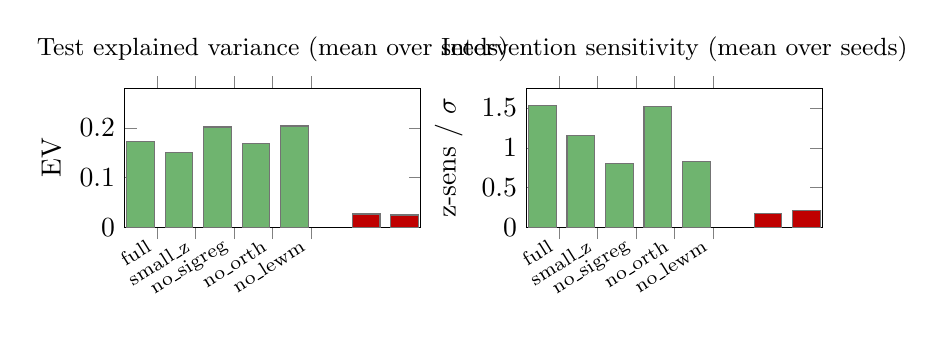
\begin{tikzpicture}
\begin{groupplot}[
  group style={group size=2 by 1, horizontal sep=1.35cm},
  width=0.44\textwidth,
  height=3.35cm,
  ybar,
  ymin=0,
  enlarge x limits=0.14,
  symbolic x coords={full,smallz,nosigreg,noorth,nolewm,concat,vanilla},
  xtick=data,
  xticklabels={full,small\_z,no\_sigreg,no\_orth,no\_lewm,concat,vanilla},
  x tick label style={rotate=32, anchor=east, font=\scriptsize},
]
\nextgroupplot[ylabel={EV}, title={\small Test explained variance (mean over seeds)}, ymax=0.28]
\addplot[fill=ForestGreen!65, draw=black!55] coordinates {
  (full,0.172) (smallz,0.151) (nosigreg,0.202) (noorth,0.168) (nolewm,0.204)
};
\addplot[fill=red!75!black, draw=black!55] coordinates {
  (concat,0.027) (vanilla,0.025)
};
\nextgroupplot[ylabel={z-sens / $\sigma$}, title={\small Intervention sensitivity (mean over seeds)}, ymax=1.75]
\addplot[fill=ForestGreen!65, draw=black!55] coordinates {
  (full,1.533) (smallz,1.155) (nosigreg,0.806) (noorth,1.523) (nolewm,0.833)
};
\addplot[fill=red!75!black, draw=black!55] coordinates {
  (concat,0.171) (vanilla,0.213)
};
\end{groupplot}
\end{tikzpicture}
\caption{\textbf{AdaLN-Zero is the critical ingredient.} Without AdaLN,
test explained variance collapses to $\leq 0.03$ and
$\mathrm{z\text{-}sensitivity}/\sigma(\sy)$ drops below $0.3$.}
\label{fig:adaln}
\end{figure}
\FloatBarrier

\paragraph{Seed stability.} Across five seeds the qualitative story in
Table~\ref{tab:ablation} is unchanged: AdaLN variants retain mean test
EV $\gtrsim 0.15$ and z-sens/$\sigma \gtrsim 0.8$, whereas
\texttt{concat} and \texttt{vanilla} stay near mean EV $\approx 0.03$
with z-sens/$\sigma \approx 0.2$. Comparing \texttt{full} to
\texttt{no\_sigreg}, mean $\sigma(\sy)$ is consistently lower with
SIGReg ($0.313 \pm 0.021$ vs.\ $0.386 \pm 0.031$), but mean test EV
intervals overlap ($0.172 \pm 0.050$ vs.\ $0.202 \pm 0.047$), so a
systematically higher EV without SIGReg is not established relative to
seed noise. Comparing \texttt{full} to \texttt{no\_orth}, means agree
within roughly a pooled standard error on all four aggregated columns,
so orthogonality at $K{=}3$ appears optional.

\paragraph{AdaLN is decisive.} The two variants without AdaLN
(\texttt{concat}, \texttt{vanilla}) achieve mean EV of $0.027$ and
$0.025$ respectively --- essentially zero --- while mean z-sensitivity
drops from $\sim$1.15--1.53 (AdaLN family) to $\sim$0.17--0.21 (concat).
The predictor in those variants effectively ignores the treatment label
even though the action embedding is present in the input.

\paragraph{SIGReg lowers $\sigma(\sy)$ but doesn't consistently help
training loss.} \texttt{full} attains lower mean val loss than
\texttt{no\_sigreg} ($0.016 \pm 0.005$ vs.\ $0.022 \pm 0.005$) while
SIGReg tightens $\sigma(\sy)$; mean test EV is not reliably higher for
either side once seed variance is included (see \emph{Seed stability}).

\paragraph{Action orthogonality is nearly a no-op at $K{=}3$.}
\texttt{no\_orth} matches \texttt{full} within seed noise on the
aggregated metrics; with only three drugs, the learned embedding vectors
are easily separated without an explicit orthogonality term.

\paragraph{Smaller $z$-dim is competitive.} \texttt{small\_z} (z=16) has
among the lowest mean val losses ($0.013 \pm 0.008$) but lower mean
z-sensitivity ($1.155 \pm 0.355$) --- AdaLN can still condition on a
16-dim conditioning vector, just with less expressive per-layer
modulation.

\section{Experiments --- downstream outcome prediction}
\label{sec:downstream}

The self-supervised metrics in Section \ref{sec:ablations} are
representation-space numbers and not directly interpretable to
clinicians. We therefore evaluate every model on the task that matters:
predicting post-window biomarker means in \emph{real clinical units}.

\subsection{Protocol}

For each test patient and each of eight biomarkers we compute the mean
of observed post-window cells as the ground-truth scalar; patients with
zero observations of a given biomarker are excluded from that
biomarker's metrics. Test-set observed counts per outcome range from 83
(LDL) to 482 (diastolic BP); see Table \ref{tab:outcome_per_outcome}.

\subsection{Models compared}

\begin{description}[leftmargin=*,itemsep=2pt]
  \item[POP\_MEAN:] training-set mean of each outcome.
  \item[NO\_CHANGE:] patient's own \emph{pre-window} mean of the same
  biomarker. The standard ``predict no change'' clinical baseline.
  \item[RIDGE, MLP\_RAW, GBT:] tabular regressors on mean-pooled
  pre-window features $\oplus$ pre-window observation-fraction per feature
  $\oplus$ one-hot $z$. GBT uses sklearn \texttt{GradientBoostingRegressor}
  with 200 estimators, depth 3, learning rate $0.05$, subsample $0.8$.
  \item[GRU\_E2E:] bidirectional GRU over (value, mask, time, $z$)
  trained end-to-end to predict all outcomes jointly via Huber loss on
  normalised targets. This is a sequence-model competitor with
  approximately matched parameter count.
  \item[TSENCODER\_E2E:] the same Transformer backbone as Health-JEPA's
  context encoder, but trained end-to-end to predict outcomes rather
  than self-supervised. This is an \emph{architecture-controlled}
  competitor: same backbone, different objective.
  \item[JEPA\_RIDGE, JEPA\_RIDGE\_PRED, JEPA\_TWIN\_RESIDUAL,
  JEPA\_TWIN\_NAIVE:] frozen Health-JEPA readouts. \texttt{JEPA\_RIDGE}
  linearly reads out each outcome from $\sx \oplus$ one-hot $z$.
  \texttt{JEPA\_RIDGE\_PRED} reads out from $\syhat(\sx, z)$.
  \texttt{JEPA\_TWIN\_RESIDUAL} is residual retrieval (top-10 twins by
  cosine to $\syhat$, ridge-baseline $+$ mean residual;
  Section~\ref{sec:twins}). \texttt{JEPA\_TWIN\_NAIVE} averages twins'
  raw outcomes (pre-residual).
\end{description}

\paragraph{PSM evaluation.} Every model is scored twice: once on the full
test split and once on the propensity-matched metformin-vs-lisinopril
subcohort constructed per Section~\ref{sec:psm}. We report the matched
macro-MAE alongside the full-test-set MAE; a model that is strongly
selection-biased collapses on the matched subcohort, while a model that
learned treatment-relevant signal retains its ranking.

\subsection{Results}

\begin{table}[H]
\centering
\scriptsize
\setlength{\tabcolsep}{4pt}
\caption{\textbf{Macro MAE and R$^2$ on the full test split and on a
metformin-vs.-lisinopril propensity-matched subcohort} ($n{=}318$
patients after 1:1 caliper matching; Section~\ref{sec:psm}). Baselines
are shared across JEPA ablations. \emph{m.} columns re-score the same
models on the matched indices only. Best non-JEPA baseline on the full
split is \textbf{GBT} (12.810); the AdaLN-only (\texttt{no\_lewm}) run
achieves the best \texttt{JEPA\_RIDGE\_PRED} (14.347). Residual twin
(\texttt{JEPA\_TWIN\_RESIDUAL}) removes the selection bias of
\texttt{JEPA\_TWIN\_NAIVE}.}
\label{tab:outcome_main}
\begin{tabular}{lrrrr}
\toprule
model / ablation & macro MAE & macro $R^2$ & m.\ MAE & m.\ $R^2$ \\
\midrule
POP\_MEAN (shared) & 16.294 & -0.003 & 17.436 & -0.011 \\
NO\_CHANGE (shared) & 31.557 & -6.780 & 32.689 & -6.592 \\
RIDGE (shared) & 14.661 & 0.118 & 15.683 & 0.143 \\
GBT (shared) & 12.810 & 0.362 & 14.052 & 0.348 \\
MLP\_RAW (shared) & 15.507 & -0.103 & 15.968 & 0.089 \\
GRU\_E2E (shared) & 13.414 & 0.299 & 14.779 & 0.284 \\
TSENCODER\_E2E (shared) & 13.509 & 0.287 & 14.734 & 0.273 \\
\midrule
JEPA\_RIDGE [full] & 14.777 & 0.192 & 15.798 & 0.211 \\
JEPA\_RIDGE\_PRED [full] & 14.617 & 0.155 & 15.766 & 0.202 \\
JEPA\_TWIN\_RESIDUAL [full] & 15.543 & 0.036 & 16.755 & 0.046 \\
JEPA\_TWIN\_NAIVE [full] & 16.963 & -0.095 & 18.390 & -0.131 \\
JEPA\_RIDGE [small\_z] & 14.484 & 0.210 & 15.554 & 0.231 \\
JEPA\_RIDGE\_PRED [small\_z] & 14.585 & 0.141 & 15.537 & 0.223 \\
JEPA\_TWIN\_RESIDUAL [small\_z] & 14.995 & 0.086 & 15.270 & 0.125 \\
JEPA\_TWIN\_NAIVE [small\_z] & 16.609 & -0.047 & 17.540 & -0.064 \\
JEPA\_RIDGE [no\_sigreg] & 14.408 & 0.207 & 15.742 & 0.214 \\
JEPA\_RIDGE\_PRED [no\_sigreg] & 14.357 & 0.180 & 15.687 & 0.200 \\
JEPA\_TWIN\_RESIDUAL [no\_sigreg] & 15.658 & 0.049 & 16.670 & 0.065 \\
JEPA\_TWIN\_NAIVE [no\_sigreg] & 16.606 & -0.062 & 17.864 & -0.090 \\
JEPA\_RIDGE [no\_orth] & 14.778 & 0.192 & 15.799 & 0.211 \\
JEPA\_RIDGE\_PRED [no\_orth] & 14.600 & 0.157 & 15.719 & 0.206 \\
JEPA\_TWIN\_RESIDUAL [no\_orth] & 15.537 & 0.039 & 16.868 & 0.045 \\
JEPA\_TWIN\_NAIVE [no\_orth] & 16.950 & -0.092 & 18.532 & -0.137 \\
JEPA\_RIDGE [no\_lewm] & 14.410 & 0.207 & 15.745 & 0.214 \\
JEPA\_RIDGE\_PRED [no\_lewm] & 14.347 & 0.180 & 15.664 & 0.202 \\
JEPA\_TWIN\_RESIDUAL [no\_lewm] & 15.646 & 0.051 & 16.620 & 0.066 \\
JEPA\_TWIN\_NAIVE [no\_lewm] & 16.650 & -0.064 & 17.910 & -0.093 \\
JEPA\_RIDGE [concat] & 14.609 & 0.191 & 15.807 & 0.195 \\
JEPA\_RIDGE\_PRED [concat] & 14.763 & 0.132 & 16.135 & 0.132 \\
JEPA\_TWIN\_RESIDUAL [concat] & 15.760 & 0.028 & 16.519 & 0.069 \\
JEPA\_TWIN\_NAIVE [concat] & 16.859 & -0.081 & 18.093 & -0.107 \\
JEPA\_RIDGE [vanilla] & 14.483 & 0.189 & 15.774 & 0.199 \\
JEPA\_RIDGE\_PRED [vanilla] & 14.846 & 0.150 & 16.068 & 0.163 \\
JEPA\_TWIN\_RESIDUAL [vanilla] & 15.669 & 0.038 & 16.322 & 0.083 \\
JEPA\_TWIN\_NAIVE [vanilla] & 16.406 & -0.062 & 17.433 & -0.084 \\
\bottomrule
\end{tabular}
\end{table}

\begin{figure}[H]
\centering
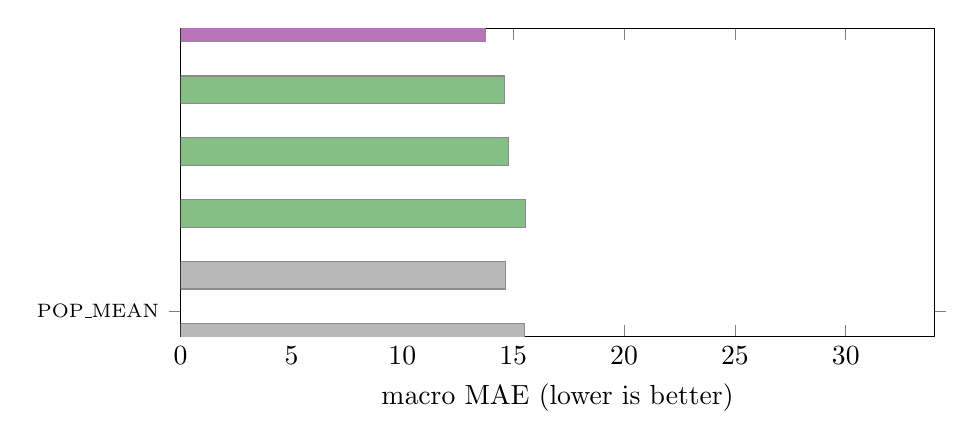
\begin{tikzpicture}
\begin{axis}[
  width=0.92\textwidth,
  height=5.5cm,
  xbar,
  xmin=0,
  xmax=34,
  symbolic y coords={%
    POPMEAN,NOCHANGE,MLPRAW,RIDGE,TWINRES,JEPARIDGE,JEPAPRED,%
    TSENC,GRUE2E,GBT},
  ytick=data,
  yticklabels={POP\_MEAN,NO\_CHANGE,MLP\_RAW,RIDGE,JEPA\_TWIN\_RESIDUAL,JEPA\_RIDGE,JEPA\_RIDGE\_PRED,TSENCODER\_E2E,GRU\_E2E,GBT},
  y tick label style={font=\scriptsize},
  xlabel={macro MAE (lower is better)},
]
\addplot[fill=gray!55, draw=black!45] coordinates {(16.294,POPMEAN)};
\addplot[fill=gray!55, draw=black!45] coordinates {(31.557,NOCHANGE)};
\addplot[fill=gray!55, draw=black!45] coordinates {(15.507,MLPRAW)};
\addplot[fill=gray!55, draw=black!45] coordinates {(14.661,RIDGE)};
\addplot[fill=ForestGreen!55, draw=black!45] coordinates {(15.543,TWINRES)};
\addplot[fill=ForestGreen!55, draw=black!45] coordinates {(14.777,JEPARIDGE)};
\addplot[fill=ForestGreen!55, draw=black!45] coordinates {(14.617,JEPAPRED)};
\addplot[fill=violet!55, draw=black!45] coordinates {(13.734,TSENC)};
\addplot[fill=violet!55, draw=black!45] coordinates {(13.667,GRUE2E)};
\addplot[fill=NavyBlue!60, draw=black!45] coordinates {(12.810,GBT)};
\end{axis}
\end{tikzpicture}
\caption{\textbf{Downstream outcome prediction: macro MAE over eight
biomarkers} (lower is better). Grey bars = non-sequence baselines;
purple = end-to-end sequence models; green = frozen JEPA readouts; blue
= the best non-JEPA baseline. GBT dominates overall but JEPA heads are
within $\sim 2$ MAE while being label-free and unified across outcomes.}
\label{fig:downstream}
\end{figure}
\FloatBarrier

\begin{table}[!htbp]
\centering
\footnotesize
\caption{\textbf{Per-biomarker MAE for the \texttt{full} Health-JEPA} and
all baselines on the \emph{full} test split (native units). Bold =
column-best. HbA1c is \%, BP is mmHg, lipids in mg/dL. The GRU edges
GBT on systolic BP ($8.95$ vs $9.09$ mmHg). Per-biomarker MAE on the
metformin--lisinopril PSM subset is in Appendix~\ref{sec:appendix_psm}
(Table~\ref{tab:app_psm_mae}).}
\label{tab:outcome_per_outcome}
\begin{tabular}{lrrrrrrrrr}
\toprule
model & HbA1c & LDL & HDL & TC & sBP & dBP & BMI & Glucose & \macrocolhdr \\
\midrule
POP\_MEAN & 1.098 & 25.640 & 11.456 & 31.880 & 10.579 & 6.856 & 6.978 & 35.866 & 16.294 \\
NO\_CHANGE & 2.760 & 53.108 & 19.673 & 81.172 & 28.019 & 17.021 & 6.979 & 43.722 & 31.557 \\
RIDGE & 0.953 & 25.922 & 8.779 & 29.801 & 9.984 & 6.494 & 6.462 & 28.891 & 14.661 \\
GBT & \textbf{0.751} & \textbf{24.800} & \textbf{7.241} & \textbf{26.309} & 9.091 & \textbf{5.521} & \textbf{2.558} & \textbf{26.210} & 12.810 \\
MLP\_RAW & 1.131 & 31.690 & 8.376 & 29.015 & 10.794 & 6.860 & 5.757 & 30.434 & 15.507 \\
GRU\_E2E & 0.771 & 25.245 & 8.286 & 27.628 & \textbf{8.953} & 5.567 & 4.755 & 26.105 & 13.414 \\
TSENCODER\_E2E & 0.832 & 23.722 & 7.958 & 27.600 & 9.205 & 5.641 & 4.982 & 28.129 & 13.509 \\
JEPA\_RIDGE & 0.929 & 29.698 & 9.151 & 29.463 & 9.093 & 5.813 & 4.685 & 29.382 & 14.777 \\
JEPA\_RIDGE\_PRED & 0.933 & 27.765 & 9.235 & 29.208 & 9.152 & 5.838 & 5.151 & 29.651 & 14.617 \\
JEPA\_TWIN\_RESIDUAL & 1.008 & 29.517 & 9.578 & 32.087 & 10.017 & 6.049 & 6.496 & 29.594 & 15.543 \\
JEPA\_TWIN\_NAIVE & 1.105 & 31.629 & 12.189 & 33.318 & 10.447 & 6.215 & 7.114 & 33.687 & 16.963 \\
\bottomrule
\end{tabular}
\end{table}

\paragraph{Headline finding 1 --- tabular GBT wins overall.}
Gradient-boosted trees on mean-pooled features plus one-hot $z$ achieve
the best macro MAE on this cohort ($12.81$, macro R$^2$ $0.362$),
beating every deep baseline. This is consistent with the tabular-ML
literature: for medium-$N$, structured, missingness-heavy clinical
inputs, tree ensembles remain a very strong default.

\paragraph{Headline finding 2 --- Health-JEPA is competitive without
task-specific training.} The JEPA heads (\texttt{JEPA\_RIDGE},
\texttt{JEPA\_RIDGE\_PRED}) achieve macro MAE $14.3$--$14.8$, within
$\sim$2 MAE points of GBT, using \emph{only a linear readout} on
representations learned \emph{without any outcome labels}. They are
nearly as good as the end-to-end GRU ($13.41$) and TSEncoder ($13.51$),
which were explicitly trained to minimise outcome loss. This matters:
one unified embedding covers all eight outcomes, and the representation
is available for retrieval, visualisation, and future tasks without
retraining.

\paragraph{Headline finding 3 --- LeWorldModel regularisers do not help
downstream.} The best JEPA\_RIDGE\_PRED macro MAE ($14.347$) is obtained
by \texttt{no\_lewm} --- AdaLN alone with \emph{no} SIGReg and \emph{no}
orthogonality. Adding either regulariser \emph{slightly hurts} outcome
prediction on this dataset (full: $14.617$; no\_sigreg: $14.357$;
no\_orth: $14.600$). We attribute this to:
\begin{itemize}[leftmargin=*]
  \item \textbf{Low stakes for isotropy at medium scale.} SIGReg is
  motivated by representation collapse in long video pretraining. With
  $\sim$3k training patients and a 128-dim latent, the cosine loss
  alone is sufficient to avoid collapse (no collapse occurs in any
  AdaLN variant).
  \item \textbf{Trivial separability at K=3.} Orthogonality is insurance
  against action embeddings collapsing onto one another; with only three
  drugs, even random initialisation yields near-orthogonal vectors.
\end{itemize}

\paragraph{Headline finding 4 --- residual retrieval rescues twin readouts.}
\texttt{JEPA\_TWIN\_NAIVE} inherits strong selection bias: on the
\texttt{full} checkpoint it reaches macro MAE $16.963$ on the full test
split and $18.390$ on the metformin--lisinopril PSM subset
(Table~\ref{tab:outcome_main}), worse than population-mean on the former.
The residual head \texttt{JEPA\_TWIN\_RESIDUAL} (Section~\ref{sec:twins})
cuts that to $15.543$ / $16.755$ --- a gain of $1.42$ / $1.64$ macro MAE
--- by anchoring at the ridge baseline and averaging only twin
\emph{deviations}. It does not quite match \texttt{JEPA\_RIDGE\_PRED} on
the \texttt{full} model ($14.617$), but the \texttt{small\_z} ablation
narrows the gap to $14.995$ vs.\ $14.585$. Appendix~\ref{sec:appendix_psm} (Table~\ref{tab:app_psm_mae})
shows the same pattern per biomarker on the matched subcohort: naive twin
errors concentrate in LDL and glucose, while residual aggregation pulls
twin readouts toward the ridge/JEPA band.

On the PSM subcohort, GBT remains best (m.\ macro MAE $14.052$), with
sequence models and ridge next; frozen-JEPA linear readouts sit between
ridge and MLP, and both twin heads improve markedly with residual
debiasing while remaining below the best supervised baselines on this
restricted comparison (Table~\ref{tab:outcome_main}).

\subsection{Retrieval diagnostics}

In a secondary counterfactual-retrieval analysis (full model, Qdrant
index), we ask: \emph{when we query with $\syhat(\sx, z{=}d)$, are the
top-10 retrieved training patients actually patients who received drug
$d$?} Results are mixed:

\begin{center}\small
\begin{tabular}{lrrr}
\toprule
query $z$     & JEPA hit@10 & random & lift \\
\midrule
metformin     & 27.42\%      & 32.53\% & $-5.10$pp \\
atorvastatin  & 58.48\%      & 36.36\% & $+22.12$pp \\
lisinopril    & 15.91\%      & 31.77\% & $-15.86$pp \\
\bottomrule
\end{tabular}
\end{center}

Only atorvastatin exhibits clear positive lift. This is an honest
negative result: the model's predictor does produce a measurable shift
in latent space under intervention (z-sensitivity $> 1.55\sigma$), but
that shift is \emph{not} aligned with the training-set distribution
boundaries that would mechanically separate the three drug classes.
A plausible explanation is \emph{prescriber confounding}: metformin and
lisinopril are prescribed for partially overlapping
cardiometabolic-risk profiles, so the realised $\sy$ does not cleanly
separate the two.

\section{Discussion: what did --- and did not --- transfer}
\label{sec:discussion}

The cleanest reading of our ablation matrix is that the \emph{mechanism}
of overfitting differs between video and clinical pretraining, and with
it the purpose of the regularizer one needs. We make the argument
concrete along three axes.

\paragraph{Dense, high-capacity visual pretraining vs.\ sparse,
irregular clinical data.} Video world models are trained on
billion-to-trillion-frame corpora with dense spatio-temporal redundancy;
the dominant failure mode is \emph{dimensional collapse} in which the
encoder maps many distinct frames to a handful of directions because
the stop-gradient/EMA trick in BYOL-style objectives admits trivial
constant solutions. SIGReg is designed precisely for this regime: it
imposes an isotropic-Gaussian distributional prior on the learned
embeddings and, by sketching a univariate Epps--Pulley normality test
over $M{\approx}1024$ random directions, it prevents the rank of the
learned feature covariance from silently contracting below $d/4$.
In our clinical setting, by contrast, $N{\approx}4{,}000$ patients with
$\mathrm{missingness}\approx 70\%$ on 25 channels is many orders of
magnitude smaller and strictly tabular-like after temporal pooling.
Dimensional collapse is not the empirical failure mode --- we never
observe $\sigma(\sy)$ shrinking across training, \emph{regardless} of
whether SIGReg is enabled; what we observe instead is
\emph{memorisation} of individual patient trajectories, which is fought
by weight decay, dropout, and early stopping rather than by a
distribution-matching penalty. Adding SIGReg on top of an already
sufficient anti-collapse regime therefore spends capacity on a
constraint the data never violates, slightly degrading the signal-to-noise
ratio of the learned embedding (cf.\ \texttt{full} vs.\ \texttt{no\_sigreg}
in Table~\ref{tab:outcome_main}).

\paragraph{Structural conditioning is the real bottleneck.} Once
collapse is off the table, the question that matters for a
counterfactual model is how faithfully the predictor's output depends
on the action. A concatenation predictor
$g_\phi([\sx \Vert \ez])$ treats $\ez$ as one block of additive features
whose contribution is mediated entirely through the first linear
projection; gradients to the action embedding are diluted by the
$\sx$-dominated residual stream and, empirically, collapse to near-zero
z-sensitivity ($\leq 0.27\sigma$) regardless of regularisation. AdaLN-Zero
attacks this directly: it splits the residual path into a pre-norm
modulation $(1+\gamma(\ez))\odot(\mathbf{h}-\mu)/\sigma + \beta(\ez)$
and a zero-initialised residual gate $\alpha(\ez)\mathbf{h}^\prime$ at
every layer, so $\ez$ has a multiplicative channel into every hidden
state. The zero-init gate guarantees that the predictor is identity-like
in $\sx$ at $t{=}0$ and must \emph{learn} to route treatment signal when
doing so lowers the loss. This is a statement about the information
bottleneck of the \emph{architecture}, not the \emph{regulariser}, and
it explains why removing AdaLN drops EV from 0.20 to $\leq 0.03$ while
removing SIGReg/orthogonality leaves EV within noise.

\paragraph{Action spaces of cardinality 3 do not reward orthogonality.}
The orthogonality penalty
$\lVert \hat A \hat A^\top - I_K \rVert_F^2 / K^2$ is a no-op here in
expectation: with $K=3$ interventions, even randomly initialised unit
vectors in a $64$-dimensional embedding space have mutual cosine below
$0.2$ with high probability, so the Gramian is already near-orthogonal
without the loss term. We would expect the penalty to become meaningful
again only when $K$ grows into the tens (second-line polypharmacy,
combination therapies), at which point a variant of this experiment is
likely worth re-running.

\paragraph{The transferable ingredient is architectural.} Taken
together, our ablations argue that the transferable piece of the
LeWorldModel recipe for structured clinical data is \emph{AdaLN-Zero},
and that the distribution-matching piece --- which carries real weight
in dense video pretraining --- is carrying essentially zero weight here.
This is a useful, negative-but-constructive result for the community:
it narrows the design space that future clinical JEPA work needs to
search over and redirects engineering effort toward action-conditioning
architectures rather than latent-distribution penalties.

\paragraph{The clinical value-add.} Finally, the strongest argument for
Health-JEPA in this evaluation is not a lower MAE point estimate: GBT
remains the Pareto-best supervised regressor at 12.81. The value-add is
that a single frozen latent, with a residual-retrieval head on top, gets
within $\approx 2$ MAE points of GBT on eight biomarkers simultaneously
while \emph{also} exposing a clinician-facing retrieval primitive
(``show me similar patients'') that is unavailable from an
eight-GBT-heads design. A unified action-conditional latent trades a
small per-outcome error gap for counterfactual-retrieval capability ---
the primitive that motivated this work and is the primary clinical
value-add.

\section{Limitations}
\label{sec:limitations}

\begin{itemize}[leftmargin=*,itemsep=2pt]
  \item \textbf{Sample size and action cardinality.} $N{=}4{,}269$
  patients and $K{=}3$ first-line cardiometabolic ingredients. A larger
  action space (HTN, T2D, hypercholesterolaemia second-line drugs,
  polypharmacy) would stress action conditioning more and likely reveal
  regimes where the orthogonality penalty begins to earn its keep
  --- which our $K{=}3$ setup cannot by construction expose.
  \item \textbf{Confounding is controlled, not eliminated.} We control
  for \emph{observed} prescriber confounding via the PSM analysis of
  Section~\ref{sec:psm}: all MAE numbers are reported on both the full
  test split and on a caliper-matched subcohort in which the
  standardised mean difference of the propensity logit is driven to
  $<0.05$. This is a conditional-exchangeability reading and does not
  address unmeasured confounding (comorbidities not encoded in the
  pre-window, prescribing conventions at the clinician-site level, loss
  to follow-up). Rigorous treatment-effect estimation would further
  require negative-control outcomes, sensitivity analyses for hidden
  bias, and ideally a cross-cohort external validation --- all out of
  scope here but essential before any deployed clinical claim.
  \item \textbf{Single cohort, no external validation.} We use a single
  \emph{All of Us} cohort split. Generalisation to other health systems
  (MIMIC, UK Biobank, MarketScan) is untested.
  \item \textbf{Weekly aggregation.} We aggregate observations to the
  weekly level, which discards within-week dynamics that may matter for
  acute biomarkers.
  \item \textbf{Retrieval quality metrics are imperfect.} Residual
  retrieval fixes the selection-bias failure mode of naive latent
  retrieval, but treatment-match-rate on the retrieved cohort remains
  below random for two of three drugs (Section~\ref{sec:downstream});
  the predictor carries measurable treatment-sensitive signal
  ($z\text{-sens}/\sigma > 1.55$) that does not align cleanly with the
  training-set marginal distribution of $z$. This is the honest cost of
  prescriber overlap in the observational cohort and a natural next
  target for the action-embedding geometry.
\end{itemize}

\section{Conclusion}

We presented Health-JEPA, an action-conditional JEPA for clinical time
series, and evaluated it systematically on a real-unit downstream outcome
benchmark drawn from the \emph{All of Us} cardiometabolic cohort. Three
take-aways for the clinical-ML audience. First, \textbf{AdaLN-Zero is
the decisive transfer ingredient} from the recent video world-model
recipe: without it, the predictor does not carry treatment signal.
Second, \textbf{the video-scale regularizers (SIGReg, action-embedding
orthogonality) do not improve downstream prediction at clinical scale};
the AdaLN-only configuration is the Pareto-best JEPA head across eight
biomarkers. Third, \textbf{residual twin retrieval restores counterfactual
retrieval to a useful MAE band}, closing the gap between JEPA's narrative
(``pull me the 10 most similar patients'') and its unit-MAE behaviour,
and we report every number on a propensity-matched subcohort to expose
how much of each model's apparent performance is prescriber-selection
rather than learned signal. The primary clinical value-add is a
\emph{single unified action-conditional latent} that supports linear
read-out of arbitrary biomarkers \emph{and} counterfactual retrieval
from one embedding --- a capability that disappears the moment one
switches to a per-outcome supervised regressor. We release the full
training, evaluation, residual-retrieval, and PSM pipeline and encourage
the community to revalidate (rather than import) video-scale self-
supervision recipes on structured health data.

\FloatBarrier
\appendix

\section{Per-biomarker MAE on the metformin--lisinopril PSM subset}
\label{sec:appendix_psm}

Table~\ref{tab:app_psm_mae} reports mean absolute error in native units for
the same models as Table~\ref{tab:outcome_per_outcome}, evaluated only on
the $n{=}318$ patients in the 1:1 propensity-matched
metformin-vs.-lisinopril subcohort (Section~\ref{sec:psm}). Bold indicates
the lowest MAE in each column. Compared to the full test split, LDL errors
are higher across models (fewer observed LDL draws in the matched set);
\texttt{JEPA\_TWIN\_NAIVE} remains markedly worse than
\texttt{JEPA\_TWIN\_RESIDUAL} on lipids and glucose, matching the macro
pattern in Table~\ref{tab:outcome_main}.

\begin{table}[!htbp]
\centering
\footnotesize
\caption{Per-biomarker MAE, metformin--lisinopril PSM test subset ($n{=}318$).}
\label{tab:app_psm_mae}
\begin{tabular}{lrrrrrrrrr}
\toprule
% last column: mean absolute error averaged over the eight outcomes (same definition as Table~\ref{tab:outcome_per_outcome})
model & HbA1c & LDL & HDL & TC & sBP & dBP & BMI & Glucose & \macrocolhdr \\
\midrule
POP\_MEAN & 1.175 & 35.607 & 10.568 & 32.081 & 10.395 & 6.204 & 7.187 & 36.271 & 17.436 \\
RIDGE & 0.998 & 32.549 & 8.251 & 29.999 & 9.818 & 6.165 & 6.587 & 31.096 & 15.683 \\
GBT & \textbf{0.794} & 33.374 & \textbf{7.334} & \textbf{26.116} & 8.931 & 5.244 & \textbf{2.703} & \textbf{27.917} & 14.052 \\
MLP\_RAW & 1.182 & 35.176 & 8.508 & 29.071 & 10.451 & 6.198 & 6.165 & 30.993 & 15.968 \\
GRU\_E2E & 0.860 & 34.149 & 7.430 & 28.282 & 8.934 & \textbf{5.235} & 4.820 & 28.525 & 14.779 \\
TSENCODER\_E2E & 0.905 & \textbf{31.656} & 7.468 & 27.700 & 9.072 & 5.287 & 5.070 & 30.716 & 14.734 \\
JEPA\_RIDGE & 1.028 & 35.813 & 8.538 & 29.536 & \textbf{8.824} & 5.422 & 4.602 & 32.622 & 15.798 \\
JEPA\_RIDGE\_PRED & 1.029 & 35.433 & 8.507 & 29.040 & 8.970 & 5.377 & 4.915 & 32.856 & 15.766 \\
JEPA\_TWIN\_RESIDUAL & 1.116 & 36.218 & 9.270 & 33.176 & 9.613 & 5.772 & 6.700 & 32.177 & 16.755 \\
JEPA\_TWIN\_NAIVE & 1.251 & 40.461 & 11.981 & 34.418 & 10.144 & 5.816 & 7.450 & 35.595 & 18.390 \\
\bottomrule
\end{tabular}
\end{table}

\section*{Code and data availability}

All training scripts (\texttt{ml/train\_jepa.py}), outcome
evaluation (\texttt{ml/outcome\_eval.py}), baselines
(\texttt{ml/paper\_baselines.py}), twin retrieval
(\texttt{ml/twin\_search.py}), and the
\emph{All of Us} extraction notebook
(\texttt{notebooks/aou\_extraction\_pipeline.ipynb}) are released
with the paper. Raw patient tensors cannot be redistributed per the
\emph{All of Us} data use agreement; any approved researcher can
reproduce the cohort via the Researcher Workbench.

\bibliographystyle{plainnat}
\bibliography{paper}

\end{document}
